% This is samplepaper.tex, a sample chapter demonstrating the
% LLNCS macro package for Springer Computer Science proceedings;
% Version 2.20 of 2017/10/04
%
\documentclass[runningheads]{llncs}
%
\makeatletter
\usepackage[algoruled,boxed,lined]{algorithm2e}
\makeatletter
\g@addto@macro{\@algocf@init}{\SetKwInOut{Parameter}{Parameters}}
\makeatother
\usepackage{amsmath}
\usepackage{amssymb}

% \usepackage{graphicx}\usepackage{draftwatermark}
% \SetWatermarkText{\textsc{Draft}}

% -------------------- My Packages -------------------- %
\usepackage{hyperref}
\usepackage{xcolor}
\usepackage[utf8]{inputenc}
\usepackage{csquotes}

\usepackage{fontspec}
\setmonofont{Roboto Mono}
\usepackage{minted}

% Draw neural network
\usepackage{tikz}

\usepackage{fancyref}
\let\oldfref\fref
\renewcommand{\fref}[1]{[\oldfref{#1}]}

%---------- Ich bin ein verdammter Künstler ----------
\usepackage{listings}
\definecolor{maroon}{RGB}{128, 0, 0}
\definecolor{pinegreen}{RGB}{1, 121, 111}
\definecolor{darkmidnightblue}{RGB}{0, 51, 102}
\definecolor{rwthblue}{RGB}{0, 84, 159}
% www.colorhexa.com for color references

% Quiet Light
\definecolor{background}{HTML}{f5f5f5}
\definecolor{keyword}{HTML}{4b83cd}
\definecolor{constant}{HTML}{ab6526}
\definecolor{function}{HTML}{aa3731} % bold
\definecolor{comment}{HTML}{aaaaaa} % italic
\definecolor{string}{HTML}{448c27}

% ---------- Hyperref -----------
\hypersetup{colorlinks=true,
            breaklinks=true,
            urlcolor=rwthblue,
            linkcolor=rwthblue,
            citecolor=rwthblue}
\def\UrlBreaks{\do\/\do-}
% -------------------------------

\newcommand{\fat}[1]{\textbf{#1}}

% ------------------ End My Packages ------------------ %

% Used for displaying a sample figure. If possible, figure files should
% be included in EPS format.
%
% If you use the hyperref package, please uncomment the following line
% to display URLs in blue roman font according to Springer's eBook style:
% \renewcommand\UrlFont{\color{blue}\rmfamily}
% I don't really care.
\renewcommand\UrlFont{\rmfamily}


\begin{document}
%
\title{Back-Propagation and Algorithms for Training Artificial Neural Networks}
%
\titlerunning{Back-Propagation and Algorithms for Training Artificial Neural Networks}
% If the paper title is too long for the running head, you can set
% an abbreviated paper title here
%
\author{Gero F. Kauerauf}
%
\authorrunning{Kauerauf}
% First names are abbreviated in the running head.
% If there are more than two authors, 'et al.' is used.
%
\institute{RWTH Aachen University\\ \email{gero.kauerauf@rwth-aachen.de}} 
%
\maketitle              % typeset the header of the contribution
%
\begin{abstract}
    \textsc{Todo} % Todo
\keywords{Deep Learning \and Back-Propagation \and Stochastic Gradient Descent \and TensorFlow}
\end{abstract}
%
%
%

% Introduction
% Section - Introduction
\section{Introduction}
\label{sec:introduction}

In this paper, we elaborate on the main algorithms used for training neural networks.
We especially lay focus on \emph{feedforward networks} and \emph{supervised learing}, for which we describe these algorithms in great detail.
For better understanding, this paper itself is structured in the same order the algorithms and methods to train are used in.
Key elements are:
\begin{itemize}
    \item Structure of \emph{feedforward networks} and \emph{forward propagation}
    \item \emph{Cost functions} and \emph{computational graphs} for these networks
    \item \emph{Backward-propagation}
    \item \emph{Stochastic gradient descent}
\end{itemize}
We make use of examples and graphics at key points for better understanding.
Furthermore, we have simplified unnecessary complex practical parts, that are not essential for a fundamental understanding.
This paper is mostly based on the standard textbook by \textbf{Goodfellow et al.} \cite{Goodfellow-et-al-2016}.
Sample citation \cite{Goodfellow-et-al-2016}.

% Section - Problem Description
\section{Problem description}
\label{sec:problem-description}

Since computers are getting better every year, one would expect that we could solve more and more problems.
This may be true in some fields, however, there are still problems that are very hard to solve.

Oftentimes, these problems are the ones that are hard to describe mathematically.
Take for example an image of a \emph{cat} and a \emph{dog}.
A human can intuitively recognize a cat on an image and is able to distinguish between those two animals with ease.
However, up to this day, it is not possible to describe the key characteristics of a \emph{cat} mathematically, 
in such a way, that one can build an algorithm that solves this problem.

Another class of problems is the one with problems that can be described mathematically perfectly but are too complex.
These are for example games like chess.
We have no problem with describing the rules of chess.
However, due to the sheer amount of possible moves and positions in chess, we have trouble analyzing games perfectly.
Writing an algorithm that \enquote{brute-forces} a game of chess is no problem, but in practice our computers are too slow.
Even worse, computers might never be fast enough!

This is where \emph{neural networks} come into play.
For these kinds of problems, they are currently the best solution we have.

% Introduction to Feedforward Networks
% Section - Feedforward networks
\section{Feedforward Networks}
\emph{Deep feedforward networks}, also called \emph{feedforward neural networks} or \emph{multilayer perceptrons} (MLPs) are are basic deep learning models.
Their main purpose is to approximate some kind of function \(f^*(x)\).
Take for example a classification function \(y = f^*(x)\), where every input \(x\) maps to a class \(y\).
A feedforward network now aims to learn the best parameters \(\Theta\) for a function \(y = f(x, \Theta)\) that approximates \(f^*(x)\).

These models are \emph{networks} due to the fact that they can be represented by \emph{directed graphs}.
One of those \emph{graphs} models the consecutive execution of functions whose composition is \(f\).
They are called \emph{feedforward networks} because the input \(x\) flows through these functions without any \emph{feedback} connections.
This means that the graph is \emph{acyclic}.
If the graph is \emph{not acyclic} and therefore \(feedback\) connections exist, we speak of \emph{recurrent neural networks}.

For example let \(f(x) = (f^3 \circ f^2 \circ f^1)(x) = f^3(f^2(f^1(x)))\).
We now define the \emph{depth} of a \emph{feedforward network} \(f\) as the number of functions that compose it.
Our example has a \emph{depth} of \(3\).
These kind of chains are very typical in \emph{neural networks}, as each function in the chain represents a layer in the \emph{directed acyclic graph}.
The last element of the chain (in our example \(f^1\)) and therefore the last layer in the graph is called the \emph{output layer} as it maps the input \(x\) to its final value.
If we think of \(f\) as a classifier function the elements of the \emph{codomain} of \(f^1\) are the classes.
Likewise, the elements of the \emph{domain} of the first function in the chain (in our example \(f^3\)) are the inputs of the network.
The first layer is called \emph{input layer}.
Layers between the \emph{input} and \emph{output} layer are called \emph{hidden layers}.

\subsection{Feedforward network graphs}
As proposed earlier we can also think of \emph{neural networks} as \emph{acyclic directed graphs}.
Loosely inspired by neuroscience, \emph{neurons} are interpreted as \emph{nodes} and \emph{synapses} as \emph{edges}.
Each \emph{node} now receives input from an arbitrary amount of neurons in the previous layer and computes an output with its own activation function.
An \emph{edges} on the other hand has a scalar \emph{weight}.
These \emph{weights} are now what can be adjusted to changed the output of the neural network.

It is shown that in most feedforward networks a \emph{rectifier linear units} (reLU) (\(f(x) = \text{max}(0, x)\)) activation function works best. \cite{Nair-Hinton} \cite{inproceedings}
However, in certain cases other activation functions might perform better.
Such would be for example the \emph{swish} activation function (\(f(x) = x * \text{sigmoid}(x)\)), that tends to perform better than reLU on deeper models. \cite{DBLP:journals/corr/abs-1710-05941}

% Small sample neural network graph
\begin{figure}[H]
    \centering
    \label{fig:dnn-example}
    
    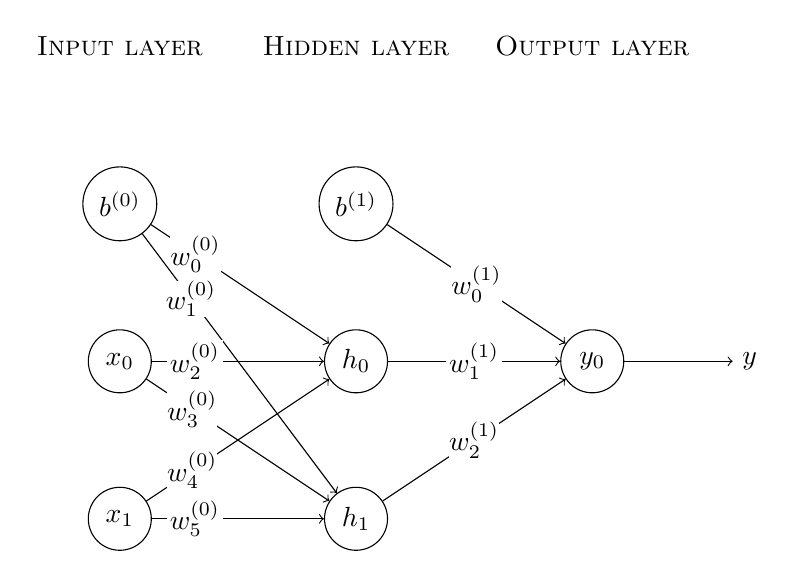
\begin{tikzpicture}
        \def\vert{2}
        \def\hori{3}
        \tikzstyle{place}=[circle, draw=black, minimum size=8mm]
        \tikzstyle{label}=[inner sep=0pt, fill=white]
        
        % Input
        \draw node at (0 * \hori, 4 * \vert) [black, ] {\textsc{Input layer}};
        
        \draw node at (0 * \hori, 3 * \vert) [place] (input_0) {$b^{(0)}$};	
        \draw node at (0 * \hori, 2 * \vert) [place] (input_1) {$x_0$};	
        \draw node at (0 * \hori, 1 * \vert) [place] (input_2) {$x_1$};
        
        
        % Hidden
        \draw node at (1 * \hori, 4 * \vert) [black, ] {\textsc{Hidden layer}};
        
        \draw node at (1 * \hori, 3 * \vert) [place] (hidden_0) {$b^{(1)}$};
        \draw node at (1 * \hori, 2 * \vert) [place] (hidden_1) {$h_0$};	
        \draw node at (1 * \hori, 1 * \vert) [place] (hidden_2) {$h_1$};	
        
        % Output
        \draw node at (2 * \hori, 4 * \vert) [black, ] {\textsc{Output layer}};
        
        \draw node at (2 * \hori, 2 * \vert) [place] (output_0) {$y_0$};
        
        % Out
        \node at (8, 2 * \vert) [black, ] (out_0) {$y$};
		
        % Input -> Hidden
        % \foreach \i in {0,...,1}
        %  	 \foreach \j in {1,...,2}
        %		 \draw [->] (input_\i) to node[near start, below] {$w_{\i}^{(0)}$} (hidden_\j);
        \draw [->] (input_0) to node[label, near start] {$w_{0}^{(0)}$} (hidden_1);
        \draw [->] (input_0) to node[label, near start] {$w_{1}^{(0)}$} (hidden_2);
        \draw [->] (input_1) to node[label, near start, inner sep=1pt] {$w_{2}^{(0)}$} (hidden_1);
        \draw [->] (input_1) to node[label, near start] {$w_{3}^{(0)}$} (hidden_2);
        \draw [->] (input_2) to node[label, near start] {$w_{4}^{(0)}$} (hidden_1);
        \draw [->] (input_2) to node[label, near start, inner sep=1pt] {$w_{5}^{(0)}$} (hidden_2);
        
        
        % Hidden -> Output
        % \foreach \i in {0,...,2}
		% \foreach \j in {0,...,0}
        %    \draw [->] (hidden_\i) to node[label] {$w_{\i}^{(1)}$} (output_\j);
        \draw [->] (hidden_0) to node[label] {$w_{0}^{(1)}$} (output_0);
        \draw [->] (hidden_1) to node[label, inner sep=1pt] {$w_{1}^{(1)}$} (output_0);
        \draw [->] (hidden_2) to node[label] {$w_{2}^{(1)}$} (output_0);
        
        \foreach \i in {0,...,0}
		    \draw [->] (output_\i) to (out_\i);
        
    \end{tikzpicture}
    \caption{Example DNN with a single hidden layer}
\end{figure}

This DNN \fref{fig:dnn-example} can now also be described by its \emph{weight matrices}. 

We can represent the weights of the edges between two layers as a \emph{weight matrices} \(\fat{W} \in \mathbb{R}^{m \times n}\).
The input can be represented as a vector \({x \in \mathbb{R}^n}\).
Calculating the output of a neural network can therefore be achieved by iterative \emph{matrix-vector multiplication} and component-wise usage of the activation function on each layer.

For \fref{fig:dnn-example} the weight matrices are
\begin{equation}
    \fat{W}^{(0)} =
    \begin{pmatrix}
        w_{2}^{(0)} & w_{4}^{(0)} \\
        w_{3}^{(0)} & w_{5}^{(0)}
    \end{pmatrix}, \quad
    \fat{W}^{(1)} = 
    \begin{pmatrix}
        w_{1}^{(1)} & w_{2}^{(1)}
    \end{pmatrix}.
\end{equation}
With the corresponding bias vectors
\begin{equation}
    b^{(0)} =
    \begin{pmatrix}
        w_{0}^{(0)} \\
        w_{1}^{(0)}
    \end{pmatrix}, \quad
    b^{(1)} =
    \begin{pmatrix}
        w_{0}^{(1)}
    \end{pmatrix}.
\end{equation}
In order to get more \enquote{flexible} we add a \emph{bias} node to each layer.
This bias node always has an input of \(1\) and describes the constant in a linear equation.

Let \(f(x)\) now be the activation function and
\begin{equation}
    x =
    \begin{pmatrix}
        x_0 \\
        x_1
    \end{pmatrix},
\end{equation}
the input vector.
The output vector for \fref{fig:dnn-example} can be calculated by evaluating the following equations.
\begin{equation}
    x_0 =
    f(W^{(0)}x + b^{0}) =
    f(
    \begin{pmatrix}
        w_{2}^{(0)} & w_{4}^{(0)} \\
        w_{3}^{(0)} & w_{5}^{(0)}
    \end{pmatrix}
    \begin{pmatrix}
        x_0 \\
        x_1å
    \end{pmatrix}
    +
    \begin{pmatrix}
        w_{0}^{(0)} \\
        w_{1}^{(0)}
    \end{pmatrix}
    )
\end{equation}
\begin{equation}
    y =
    f(W^{(1)}x_0 + b^{1}) =
    f(
    \begin{pmatrix}
        w_{1}^{(1)} & w_{2}^{(1)}
    \end{pmatrix}
    x_0
    +
    \begin{pmatrix}
        w_{0}^{(1)}
    \end{pmatrix}
    )
\end{equation}
Where the activation function \(f\) is used component-wise.

% \subsection{tf.keras.Sequential}

% Introduction to Deep Learning
% Section - Deep learning
\section{Deep learning}
\label{sec:deep-learning}

% Subsection - Cost Functions
\subsection{Cost Functions}
A very important aspect of neural networks is the choice of a cost function.
In most cases we can make use of \emph{maximum likelihood} principle, because a neural network defines a distribution \(p(y \vert x ; \theta)\).xw

% Subsection - Computational Graphs
\subsection{Computational graphs}
\label{sec:computational-graphs}

Another important concept is the one of \emph{computational graphs}.
A \emph{computational graph} describes a mathematical expression.
Such a \emph{directed graph} consists out of nodes and edges.
A node represents an arbitrary variable, that may be a scalar, a vector, a matrix or of any other type.
Then there are also \emph{operations}.
An \emph{operation} can be informally described as a label on a node.
This label defines the operation that is performed on the input.
Whereas the input is given by the \emph{directed edges} to that node.
An operation can take an arbitrary amount of inputs and stores the result in its node.

An example is given by \fref{fig:comp-graph-example}.

\begin{figure}[h]
    \centering
    \label{fig:comp-graph-example}
    
    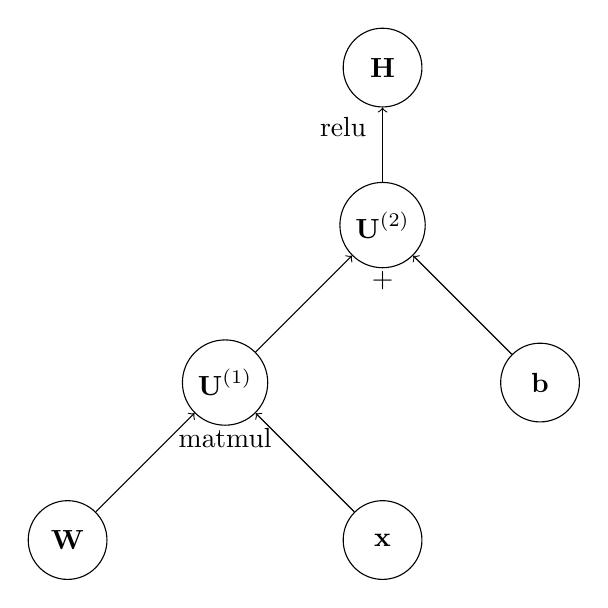
\begin{tikzpicture}
        \def\vert{2}
        \def\hori{2}
        \tikzstyle{place}=[circle, draw=black, minimum size=10mm]
        
        % Nodes
        \node[place] (w) at (0 * \hori, 0 * \vert) {\textbf{W}};
        \node[place] (x) at (2 * \hori, 0 * \vert) {\textbf{x}};
        
        \node[place, label={[shift={(0.0,-1.5)}]{\text{matmul}}}] (u1) at (1 * \hori, 1 * \vert) {$\textbf{U}^{(1)}$};
        \node[place] (b) at (3 * \hori, 1 * \vert) {\textbf{b}};
        
        
        \node[place, label={[shift={(0.0,-1.5)}]{\text{+}}}] (u2) at (2 * \hori, 2 * \vert) {$\textbf{U}^{(2)}$};
        
        \node[place, label={[shift={(-0.5,-1.5)}]{\text{relu}}}] (h) at (2 * \hori, 3 * \vert) {\textbf{H}};
        
        % Edges
        \draw [->] (w) to (u1);
        \draw [->] (x) to (u1);

        \draw [->] (u1) to (u2);
        \draw [->] (b) to (u2);
        
        \draw [->] (u2) to (h);
        
    \end{tikzpicture}
    \caption{Example of a computational graph}
\end{figure}
This specific computational graph describes the expression \(H = \max\{0, \fat{W}\fat{x} + \fat{b}\}\), 
where \enquote{relu} refers to the rectifier linear unit function \(f(x) = \max\{0, x\}\).
Therefore this describes the forward propagation of a vector \fat{x} through one layer, where the activation function (\enquote{relu}) is used component-wise as introduced in \fref{sec:feedforward-networks}.

% Subsection - Back-Propagation
\subsection{Back-Propagation}
\label{sec:back-propagation}

% Subsection - Stochastic gradient descent
\subsection{Stochastic gradient descent}
\emph{Stochastic gradient descent} (SGD) is the main \emph{optimization algorithm} that is used in \emph{deep learning}.
In \emph{TensorFlow} many of the \emph{optimizers} that come within \emph{keras} are based on the SGD algorithm.

The underlying gradient descent is an iterative optimization algorithm.
Its main idea is to start at an arbitrary point and from there on step into a direction the that minimizes the function value.
This way, it gets closer to a minimum with each step.
Suppose we have a function \(f : \mathbb{R}^2 \rightarrow \mathbb{R}\) that is differentiable.
For any point \(x_0\) we can evaluate its derivative \(f^{\prime}(x_0)\).
And since the derivative describes the slope of the function, it tells us if we have to increase or decrease \(x_0\) in order to make \(f(x_0)\) smaller.

Therefore we can reduce \(f(x)\) by taking a small step into the opposite direction of the derivative \cite{cauchy}
\begin{equation}
    \label{eq:cauchy}
    f(x - \epsilon \; \text{sign}(f^{\prime}(x))) < f(x), \qquad \text{for a small enough } \epsilon.
\end{equation}

% Todo make graphic that shows x^2 and 2x and their correlation

What is shown in (fref figure above todo) and \fref{eq:cauchy} can of course be expanded to \(\mathbb{R}^n\).

Let \(x \in \mathbb{R}^n\) and \(f : \mathbb{R}^n \rightarrow \mathbb{R}^m\).
The directional derivative of \(f\) in direction \(u\), a unit vector, is the slope of \(f\) in direction \(u\).
The directional derivative of \(f(x)\) is defined as 
\begin{equation}
    \frac{\partial}{\partial \alpha} f(x + \alpha u) = u^{T} \nabla_x f(x) \big\vert_{\alpha = 0}.
\end{equation}

We would now like to know in which direction \(f\) decreases the fastest.
This can be found out by using the directional derivative.
\begin{align}
      &\min_{u, u^{T}u = 1} u^{T} \nabla_x f(x) \\
    = &\min_{u, u^{T}u = 1} \lVert u \rVert_2 \lVert \nabla_x f(x) \rVert_2 \cos \theta \\
    = &\min_{u, u^{T}u = 1} \lVert \nabla_x f(x) \rVert_2 \cos \theta,
\end{align}
where \(\text{cos } \theta\) is the angle between the gradient and \(u\).
By ignoring the gradient, which does not depend on \(u\), this simplifies further to \(\min_{u} \cos \theta\).
Since \(\cos(\pi/2) = 0\), this is minimized if the gradient and the unit vector point in opposite directions.
This means the negative gradient points the steepest way downhill.

Therefore taking a step in direction of \(-\nabla_x f(x)\) is an improvement.
It follows that
\begin{equation}
    \lVert f(x - \epsilon \; \nabla_x f(x)) \rVert < \lVert f(x) \rVert, \qquad \text{for a small enough } \epsilon,
\end{equation}
expandes the gradient descent algorithm to arbitrary dimension. This is also called \emph{method of steepest descent}.


% \subsection{tf.model}

% Section - State of the Art
\section{State of the art}
\label{sec:state-of-the-art}

Modern neural network implementations such as Keras in TensorFlow \cite{tensorflow2015-whitepaper} are used in a broad variety of fields.
They got in fact so popular, that almost everybody has heard of them.
They have been on a rise for the last 40 years and it seems like this trend is not going to stop anytime soon.
With computers getting constantly faster, the number of fields in which neural networks can be used also increases.

Especially in the last years, there has been a huge interest and development in neural networks.
Modern optimization algorithms such as \emph{Ftrl} \cite{McMahan} and new activation functions like \emph{swish} \cite{DBLP:journals/corr/abs-1710-05941} by Google are increasing the power of even more.

% Section - Conclusion
\section{Conclusion}
\label{sec:conclusion}

Neural networks are used because they are doing what other algorithms struggle with.
For certain problem classes, they are the best we currently have.
It is not a question of choice either, since there is simply no good alternative to them.
However, we should keep in mind that they should not be \enquote{over-used}.
For problems for which we have good algorithms, we do not need neural networks.

A real problem with neural networks however is their practical nature.
It is often a \enquote{trial and error} to determine what works well.
Theoretically analyzing why it works well, is most of the time incredibly laborious and very complex.

%
% ---- Bibliography ----
%
% BibTeX users should specify bibliography style 'splncs04'.
% References will then be sorted and formatted in the correct style.
%
\bibliographystyle{splncs04}
\bibliography{refs}

\end{document}
